\documentclass[11pt]{article}
\usepackage[scaled=0.92]{helvet}
\usepackage{geometry}
\geometry{letterpaper,tmargin=1in,bmargin=1in,lmargin=1in,rmargin=1in}
\usepackage[parfill]{parskip} % Activate to begin paragraphs with an empty line rather than an indent %\usepackage{graphicx}
\usepackage{amsmath,amssymb, mathrsfs, dsfont}
\usepackage{tabularx}
\usepackage[font=footnotesize,labelfont=bf]{caption}
\usepackage{graphicx}
\usepackage{xcolor}
%\usepackage[linkbordercolor ={1 1 1} ]{hyperref}
%\usepackage[sf]{titlesec}
\usepackage{natbib}
\usepackage{../../Tianpei_Report}


\begin{document}
\title{Self-study: Optimal Transport}
\author{ Tianpei Xie}
\date{Aug. 17th., 2022}
\maketitle
\tableofcontents
\newpage
\section{The problem of optimal transport}
The problem of \textbf{optimal transport} concerns about \textbf{moving} \emph{simultaneously several items} (or a continuous distribution
thereof) from one configuration onto another with the \textbf{least amount of cost} or effort. All major economic problems, in logistics, production planning or network
routing, involve moving distributions, and that thread appears in all of the seminal references on optimal transport.  Recently, OT is being applied in Machine Learning (ML). Examples include \emph{robust optimization}, \emph{Langevin Monte Carlo (LMC) sampling}, \emph{Generative Adversarial Networks (GANs)}, \emph{Nonnegative Matrix Factorization (NMF)}, semi supervised learning etc. This chapter is mainly based on journals \citep{gabriel2019computational}.

\subsection{Probability measures}
Consider the space of probability simplex $\Delta_{n}:= \{p_1, \ldots, p_n: \sum_{i=1}^{n}p_i = 1, \;\; p_i \ge 0\}$. We can define a \textbf{discrete measure} (i.e. distribution of discrete random variables)
\begin{align*}
\alpha &:= \sum_{i=1}^{n}a_i \delta_{\mb{x}_{i}}
\end{align*} where $\delta_{\mb{x}_{i}}$ is the point mass (Dirac funcation) at $\mb{x}_i$. $\mb{a} \in \Delta_{n}$. $\alpha$ can be used to describe the distribution of the mass in one location. 

We also consider the distribution on continous random variable. Specifically, we consider the set of \emph{\textbf{Radon measures}} $\cM(\cX)$ on the space $\cX$ \citep{folland1999real}. Denote $\cC(\cX)$ be the space of all continous functions $f$ on $\cX$ with compact support. By \textbf{the Riesz representation theorem}, for a positive linear functional $I$ on $\cC(\cX)$, there exists on a unique Radon measure $\alpha$ such that
\begin{align*}
I(f) &= \int_{\cX} f(x) d\alpha(x) \in \bR,  \quad\text{for all }f \in \cC(\cX)
\end{align*} If $\cX := \bR^{d}$, we have Lebesgue measure and $\int_{\cX} f(x) d\alpha(x)=\int_{\cX} f(x) \rho_{\alpha}(x) dx,  \;\; f \in \cC(\bR^{d}) $ for some density $\rho_{\alpha}= \frac{d\alpha}{dx}$. In this document, we consider only the probablity measure $\int_{\cX} d\alpha(x) = 1$ and $\alpha \in \cM_{+}(\cX)$ is positive measure, i.e. $\alpha \in \cM^{1}_{+}(\cX)$.

\subsection{Optimal assignment problem}
\subsubsection{Problem formulations}
The \textbf{Monge problem} between discrete measures consider the problem of  \textbf{pushing forward} $n$ piles of mass $\mb{a}=[a_1, \ldots, a_n]$ at one location $\mb{X} = [\mb{x}_1, \ldots, \mb{x}_{n}]$  to $m$ piles $\mb{b}=[b_1, \ldots, b_m]$ at another location  $\mb{Y} = [\mb{y}_1, \ldots, \mb{y}_{m}]$ with \emph{minimized} cost of transportation.

Specifically, given two discrete measures $\alpha = \sum_{i=1}^{n}a_i \delta_{\mb{x}_{i}}$ and $\beta := \sum_{i=1}^{m}b_i \delta_{\mb{y}_{i}}$, consider a map $T: \{\mb{x}_1, \ldots, \mb{x}_{n}\} \rightarrow \{\mb{y}_1, \ldots, \mb{y}_{m}\}$.  The \textbf{optimal assignment problem} is defined by the following optimization problem: 
\begin{align}
\min_{T}& \sum_{i}c(\mb{x}_i, T(\mb{x}_i)) \label{eqn: optimal_assignment_discrete}\\
\text{s.t. }& \mb{b}_{j} = \sum_{i: T(\mb{x}_i) = \mb{y}_{j}}\mb{a}_{i},\; \forall\, j,  \label{eqn: optimal_assignment_discrete_constraint}
\end{align}where $c(\mb{x}, \mb{y})$ is the cost of transportation between position $\mb{x}$ and $\mb{y}$. We can define  $\mb{C}_{n,m} := [C_{i,j}]_{i\in [1:n], j\in [1:m]}$, where $C_{i,j}:= c(\mb{x}_i, \mb{y}_j) \ge 0$. Note that if $n=m$, the map $T=\sigma \in \text{Perm}(n)$, where $\text{Perm}(n)$ is the set of all permutations for $[1:n]$. If $\mb{a} = \mb{b} = \frac{1}{n}\mb{1}$ is uniformly distributed, then the constraint \eqref{eqn: optimal_assignment_discrete_constraint} can be removed. We have the classical optimal assignment problem \citep{gabriel2019computational}
\begin{align}
\min_{\sigma \in \text{Perm}(n)}& \frac{1}{n}\sum_{i=1}^{n} C_{i, \sigma(i)} \label{eqn: classical_optimal_assignment}
\end{align} 

The constraint in \eqref{eqn: optimal_assignment_discrete_constraint} defines a \textbf{\emph{Push-forward operator}} for discrete measures $T_{\#}\alpha :=  \sum_{i=1}^{n}a_i \delta_{T(\mb{x}_{i})}$. Here we can define the push-forward operator for general (Radon) measures:  
\begin{definition} For a \emph{continous} map $T : \cX \rightarrow \cY$,  the \textbf{\emph{push-forward operator}} is defined as $T_{\#}: \cM(\cX) \rightarrow \cM(\cY)$ that  satisfies 
\begin{align}
\forall\, h\in \cC(\cX), \quad \int_{\cY}h(\mb{y})\; d \paren{T_{\#}\alpha}(\mb{y}) &= \int_{\cX}h(T(\mb{x}))\; d\alpha(\mb{x}). \label{eqn: def_push_forward_opt}\\
\text{or equivalently, } \quad \paren{T_{\#}\alpha}(B)&:= \alpha\paren{\set{ \mb{x}: T(\mb{x}) \in B \subset \cY }} = \alpha(T^{-1}(B))  \label{eqn: def_push_forward_opt2}
\end{align} where the \textbf{push-forward measure} $\beta := T_{\#}\alpha \in \cM(\cY)$ of some $\alpha \in  \cM(\cX)$, $T^{-1}(\cdot)$ is the pre-image of $T$, and $\cM(\cX)$ is the set of \emph{Radon measures} on the space $\cX$. 
\end{definition} Note that for positive measure $\cM_{+}(\cX)$, $T(\cM_{+}(\cX)) \subseteq \cM_{+}(\cY)$, i.e. the push-forward operator $T_{\#}$ preserves positivity and total mass. A push-forward operator is also \textbf{linear}: $T_{\#}(w_1\alpha_1 + w_2\alpha_2) = w_1 T_{\#}(\alpha_1) + w_2 T_{\#}(\alpha_2) $. The operator $T_{\#}$ pushes forward each elementary mass of a measure $\alpha$ on $\cX$ by applying the map $T$ to obtain then an elementary mass in $\cY$. 

With the definition of push-forward operator, the \textbf{Monge problem between arbitrary measures} can be formulated as
\begin{align}
\min_{T}& \int_{\cX} c(\mb{x}, T(\mb{x})) d\alpha (\mb{x}) \label{eqn: optimal_assignment_cont}\\
\text{s.t. }& \beta = T_{\#}\alpha
\end{align} where two arbitrary probability measures $(\alpha, \beta)$, supported on two spaces $(\cX , \cY)$ can be linked through a map $T : \cX \rightarrow \cY$ so that $T$ push forward the mass of $\alpha$ to $\beta$. The equality constraint with push-forward operator in fact defines the \textbf{mass conservation constraint}.

\subsubsection{Push-forward on density}
Assume that $(\alpha, \beta)$ have densities $(\rho_{\alpha}, \rho_{\beta})$ with respect to a fixed measure, and $\beta = T_{\#}\alpha$. In multivariate distribution/density, we see that $T_{\#}$ acts on a density $\rho_{\alpha}$ linearly to a density $\rho_{\beta}$ as a change of variable, i.e. 
\begin{align}
\rho_{\alpha}(\mb{x}) &= \abs{\det(T'(\mb{x}))}\rho_{\beta}(T(\mb{x}))  \label{eqn: density of push-forward distribution}\\
\abs{\det(T'(\mb{x}))} &= \frac{\rho_{\alpha}(\mb{x}) }{\rho_{\beta}(T(\mb{x})) } \nonumber
\end{align}

\subsubsection{Push-forward vs. pull-back}
\begin{figure}
\begin{minipage}[t]{1\linewidth}
  \centering
  \centerline{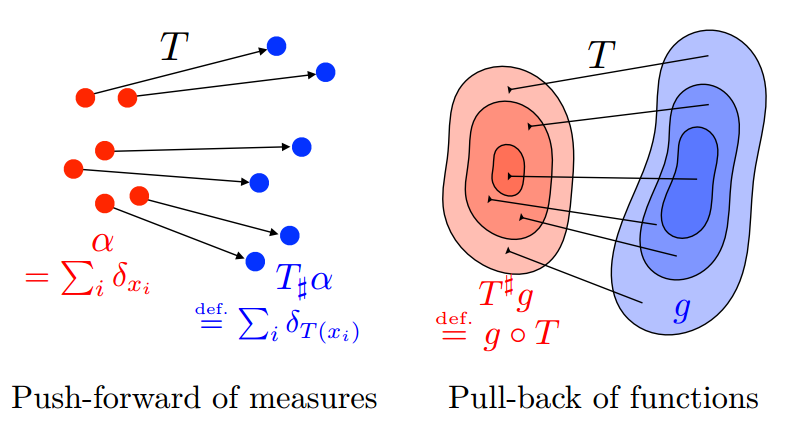
\includegraphics[scale = 0.3]{push_forward_pull_back.png}}
\end{minipage}
\caption{\footnotesize{\textbf{The comparison between push-forward operator and pull-back operator}}}
\label{fig: push_forward_pull_back}
\end{figure}
We should not be confused the\textbf{ push-forward} of \emph{\textbf{measures}} with the \textbf{pull-back} of \emph{\textbf{functions}} $T^{\#}: \cC(\cY) \rightarrow \cC(\cX)$ which corresponds to "\emph{warping}" between functions, defined as the \emph{linear} map which to $g \in \cC(\cY)$ associates $T^{\#}g = g \circ T$.  \textbf{Push-forward} and \textbf{pull-back} are actually \textbf{adjoint to one another}, in the sense that 
\begin{align}
\forall (\alpha, g) \in \cM(\cX) \times \cC(\cY): \quad \int_{\cY} g d\paren{T_{\#}\alpha}(\mb{x}) &= \int_{\cX} T^{\#}g d\alpha(\mb{x}) := \int_{\cX} g \circ T d\alpha(\mb{x}) \label{eqn: push_forward_pull_back}\\
\Leftrightarrow (T_{\#}\alpha)(A) &= \alpha(T^{-1}(A))
\end{align} Note that even if $(\alpha, \beta)$ have densities $(\rho_{\alpha}, \rho_{\beta})$ with respect to a fixed measure and $\beta = T_{\#}\alpha$, the density of push-forward measure is not equal to the pull-back of density, i.e. $\rho_{T_{\#}\alpha} \neq T^{\#}\rho_{\beta}$. The gap is the Jacobian related to change of variables.


\subsubsection{Push-forward operator for probablity measures}
Radon measures can also be viewed as representing the distributions of random variables. The distribution of random variable $X$ is a Randon measure $\alpha \in \cM_{+}^{1}(\cX)$, which is defined by $\alpha(A) := \int_A X(\omega) d\omega = \bP(X \in A)$. Following the definition above, the \underline{\textbf{distribution of}} $X$, $\alpha$, can be seen as a \underline{\textbf{push-forward} of $\bP$ by $X$}, i.e.  \underline{$\alpha = X_{\#}\bP$}. For a random variable $Y$ so that  \underline{$Y= T(X)$}, the \emph{distribution of $Y$ can be seen as a push-forward of the distribution of of X} by $T$, i.e.  \underline{$\beta = T_{\#}\alpha$}.

\subsection{Kantorovich relaxation}
\subsubsection{Optimal transport as linear programming}
The optimal assignment problem \eqref{eqn: optimal_assignment_discrete}  is \emph{\textbf{combinatorial}} and for its continous case \eqref{eqn: optimal_assignment_cont} its feasible set (the set of all push-forward operators) is \emph{\textbf{non-convex}}. Both are therefore difficult to solve when approached in their original formulation.

Kantorovich comes up with several critical relaxation: 
\begin{itemize}
\item instead of considering \emph{deterministic transport} $T$, Kantorovich considers a \textbf{\emph{probabilistic transport}} $\mb{P} \in \bR_{+}^{n \times m}$. This change allows for \underline{\emph{mass splitting}} from a source toward several targets, i.e. from one-to-one mapping to one-to-many mapping.  

\item instead of considering \emph{asymmetric} transport i.e. move mass from one location $\cX$ to another location $\cY$, Kantorovich considers a \textbf{symmetric}  transport, i.e. we can change the move direction from $\cY$ to $\cX$ and the optimal solution is unchanged. 
\end{itemize}

The \textbf{\emph{optimal transport}} under Kantorovich relaxation is formulated as a \emph{\underline{linear programming} problem}:
\begin{align}
\min_{\mb{P} \in \bR_{+}^{n \times m}} & \inn{\mb{P}}{\mb{C}} = \sum_{i,j}C_{i,j} P_{i,j} \label{eqn: optimal_transport_linear_prog}\\
\text{s.t. }&  \mb{P}\mb{1}_{m} = \mb{a} \label{eqn: optimal_transport_linear_constraint}\\
&\mb{P}^{T}\mb{1}_{n} = \mb{b}  \label{eqn: optimal_transport_linear_constraint2} \\
&P_{i,j} \ge 0 \nonumber
\end{align} where $\mb{C}_{n,m} := [C_{i,j}]_{i\in [1:n], j\in [1:m]}$,  $C_{i,j}:= c(\mb{x}_i, \mb{y}_j) \ge 0$. The \textbf{coupling matrix}  $\mb{P} = [P_{i,j}]_{n, m}$ where $P_{i,j}$ describes the amount of mass flowing from bin $i$ toward bin $j$, or from the mass found at $\mb{x}_i$ toward $\mb{y}_j$ in the formalism of
discrete measures. Denote the \textbf{optimal value} of this problem $L_{\mb{C}}(\mb{a}, \mb{b}) := \min_{\mb{P} \in U(\mb{a}, \mb{b})}  \inn{\mb{P}}{\mb{C}}$ where $U(\mb{a}, \mb{b}) := \{\mb{P} \in \bR_{+}^{n \times m}: \mb{P}\mb{1}_{m} = \mb{a}, \;\mb{P}^{T}\mb{1}_{n} = \mb{b}\}$ defines the feasible region.

It is natural to represent the optimal value $L_{\mb{C}}(\mb{a}, \mb{b})$ in terms of the discrete measures $\alpha = \sum_{i=1}^{n}a_i \delta_{\mb{x}_{i}}$ and $\beta := \sum_{i=1}^{m}b_i \delta_{\mb{y}_{i}}$, thus the \textbf{optimal transport} between $\alpha$ and $\beta$ is 
\begin{align}
\cL_{c}(\alpha, \beta) &:= L_{\mb{C}}(\mb{a}, \mb{b}) =  \min_{\mb{P} \in U(\mb{a}, \mb{b})}  \inn{\mb{P}}{\mb{C}} \label{eqn: optimal_transport_value}
\end{align} Here we emphasis the cost function $c(x, y)$.


\subsubsection{Kantorovich Relaxation is tight for optimal assignment}\label{sec: discrete_tight}
We can reformulate the original optimal assignment problem \eqref{eqn: classical_optimal_assignment} into \eqref{eqn: optimal_transport_linear_prog}. Consider the matrix representation of permuation $\sigma \in  \text{Perm}(n)$ as
\begin{align*}
\mb{P}_{\sigma} &= [ P_{i,j}]_{n \times n} \\
P_{i,j} &=  \left\{\begin{array}{cc}
 \frac{1}{n} & \text{if } j = \sigma(i) \\ 
 0 & \text{o.w. }
\end{array}\right.
\end{align*} Note that $\text{Perm}(n)$ is a symmetric group, usually denoted as $S_{n}.$ $\mb{P}_{\sigma}$ is a coupling matrix as defined in \eqref{eqn: optimal_transport_linear_prog} since each row and column only has one number $1/n$, i.e. $\mb{P}_{\sigma}\mb{1}_{n} = 1/n$ and $\mb{P}_{\sigma}^{T}\mb{1}_{n} = 1/n$. We see that \eqref{eqn: optimal_transport_linear_prog} can be converted into the classical optimal assignment problem \eqref{eqn: classical_optimal_assignment}. Note that the permutation matrix $\mb{P}_{\sigma}$ is a feasible solution,  i.e. 
\begin{align*}
L_{\mb{C}}(\mb{a}, \mb{b}) &\le \inn{\mb{P}_{\sigma}^{*}}{\mb{C}} =\min_{\sigma \in \text{Perm}(n)} \frac{1}{n}\sum_{i=1}^{n} C_{i, \sigma(i)}
\end{align*} 

Now we show that if $\mb{a} = \mb{b} = \mb{1}_{n}/n$, then solving LP \eqref{eqn: optimal_transport_linear_prog} results in the same optimal solution of \eqref{eqn: classical_optimal_assignment},  i.e. the Kantorvich relaxation is \emph{\textbf{tight}} for optimal assignment problem. 

\begin{proposition}
(\textbf{Kantorovich for matching}). If $m = n$ and  $\mb{a} = \mb{b} = \mb{1}_{n}/n$, then there exists an optimal solution for Problem \eqref{eqn: optimal_transport_linear_prog} $\mb{P}_{\sigma}$, which is a permutation matrix associated to an optimal permutation $\sigma \in \text{Perm}(n)$ for Problem \eqref{eqn: classical_optimal_assignment}.
\end{proposition}
\begin{proof}
Note that for finite-dimensional linear programming with non-empty feasible set, the optimal solution exists and it can only be found at the \emph{extreme point} of the non-empty polyhedron $U(\mb{a}, \mb{b})$. For $\mb{a} = \mb{b} = \mb{1}_{n}/n$, the feasible set $U( \mb{1}_{n}/n,  \mb{1}_{n}/n)$ is called the \textbf{Birkhoff polytope}. By Birkhoff's theorem [1946],  the set of extremal points of $U( \mb{1}_{n}/n,  \mb{1}_{n}/n)$ is equal to the set of permutation matrices. Therefore there exists a permutation $\sigma$ whose matrix representation $\mb{P}_{\sigma}$ is the optimal solution. Thus the \eqref{eqn: classical_optimal_assignment} and \eqref{eqn: optimal_transport_linear_prog} are equivalent. \qed
\end{proof}

\begin{figure}
\begin{minipage}[t]{1\linewidth}
  \centering
  \centerline{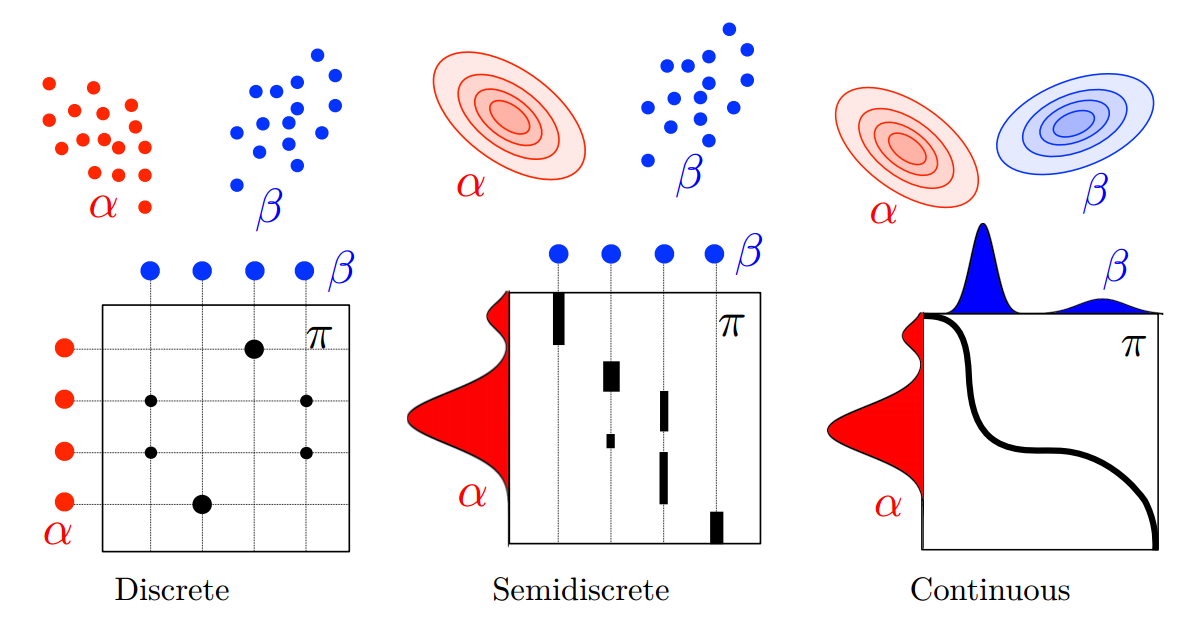
\includegraphics[scale = 0.3]{coupling_dist.png}}
\end{minipage}
\caption{\footnotesize{\textbf{The coupling matrix between discrete measures, between discrete-and-continous measures, and between continuous measures }}}
\label{fig: coupling_dist}
\end{figure}
\subsubsection{Generalization to arbitrary measures: infinite-dimension LP}
We can generalize the Kantorovich relaxation to continous measures. Let us define the set of coupling $\pi$ as
\begin{align}
U(\alpha, \beta) &:= \set{\pi \in \cM_{+}^{1}(\cX \times \cY): \;\; P_{\cX \#}\pi = \alpha, \; P_{\cY \#}\pi = \beta} := \Gamma(\alpha, \beta) \label{eqn: coupling_constraint_continous}
\end{align} Here $P_{\cX \#}$ and $P_{\cY \#}$ are the \emph{push-forwards}  of the \textbf{projections} $P_{\cX}(x, y) = x$ and $P_{\cY}(x, y) = y$. This constraint is equivalently enposing that 
\begin{align*}
\pi(A \times \cY) = \alpha(A), \;\; \pi(\cX \times B) = \beta(B),\quad \text{for any sets }A\subset \cX,\; B\subset \cY.
\end{align*}

The \textbf{Kantorovich problem between arbitrary measures} can be formulated as 
\begin{align}
\min_{\pi \in \cM_{+}^{1}(\cX \times \cY)}& \int_{\cX \times \cY} c(x, y) d \pi(x, y)  \label{eqn: optimal_transport_continuous} \\
\text{s.t. }& P_{\cX \#}\pi = \alpha,  \nonumber \\
& P_{\cY \#}\pi = \beta  \nonumber
\end{align} And the \textbf{optimal transport} is defined as the optimal value $\cL_{c}(\alpha, \beta) := \inf_{\pi \in U(\alpha, \beta)} \int_{\cX \times \cY} c(x, y) d \pi(x, y).$

The problem \eqref{eqn: optimal_transport_continuous} is a \textbf{infinite-dimensional linear programming problem} over space of measures. If $(\cX, \cY)$ are \emph{compact} spaces and $c$ is \emph{continuous}, then it is easy to show that \textbf{it always has solutions}, i.e. the feasible set $U(\alpha, \beta)  \neq \emptyset$. 

\subsubsection{Probabilistic interpretation}
Let the coupling $\pi \in \cM_{+}^{1}(\cX \times \cY)$ is the \textbf{joint probability measure} of  $(X, Y)$ over $\cX \times \cY$ and $\alpha$ and $\beta$ be the distribution of $X$ and $Y$, respectively,  the problem \eqref{eqn: optimal_transport_continuous} can be formulated as
\begin{align}
\min_{(X, Y) \sim \pi}& \E{(X,Y)}{c(X, Y)}   \label{eqn: optimal_transport_prob} \\
\text{s.t. }&  X \sim \alpha,  \nonumber \\
& Y\sim \beta  \nonumber
\end{align}

Note that the push-forward constraint states that the \emph{\textbf{marginalization}} of $\pi$ in $\cX$ and $\cY$ is equal to the distribution measure $\alpha$ and $\beta$, respectively. That is, given marginal distribution $X \sim \alpha$ and $Y \sim \beta$, we need to find $\pi$ as the joint distribution of $(X,Y)$ that match each marginal distribution, which is a natural law for joint distribution. In fact, all possible joint distribution $\pi$ in $\cX \times \cY$ that fit the marginal distribution in each random variable is a feasible solution. 


\subsection{Dual problem}
\subsubsection{Dual formulation and Kantorovich potentials}
The linear programming problems of optimal transport in \eqref{eqn: optimal_transport_linear_prog} have \textbf{dual problems}. In fact, due to \textbf{strong duality} of LP \citep{bertsimas1997introduction}, the dual problem and the primal problem share the same optimal value. 

The \underline{\textbf{dual problem}} of Kantorovich problem \eqref{eqn: optimal_transport_linear_prog} is described as below:
\begin{align}
\max_{\mb{\lambda} \in \bR^{n}, \mb{\mu} \in \bR^{m}} & \inn{\mb{\lambda}}{\mb{a}} + \inn{\mb{\mu}}{\mb{b}} \label{eqn: optimal_transport_dual}\\
\text{s.t. } & \lambda_i + \mu_{j} \le C_{i,j}\quad \forall\, i\in [1:n], j\in [1:m] \label{eqn: optimal_transport_dual_constraint}
\end{align} where $\mb{\lambda}= [\lambda_i]_{n}$, $\mb{\mu}= [\mu_{j}]_{m}$ are \textbf{dual variables} (slack variables) for marginal distribution constrain $\mb{a}$ and $\mb{b}$. We denote $\mb{\lambda}\oplus \mb{\mu}:= \mb{\lambda}\mb{1}_{m}^{T} + \mb{1}_{n}\mb{\mu}^{T} \in \bR^{n\times m}$ so that the linear constraints is $\mb{\lambda}\oplus \mb{\mu} \le \mb{C}$. Such dual variables $\mb{\lambda}$, $\mb{\mu}$ are often referred to as "\emph{\textbf{Kantorovich potentials}}." The feasible set of the dual problem is defined as 
\begin{align}
R(\mb{C}) := \set{\mb{\lambda} \in \bR^{n}, \mb{\mu} \in \bR^{m}: \mb{\lambda}\oplus \mb{\mu} \le \mb{C}} \label{eqn: optimal_transport_dual_feasible_set}
\end{align}

The relationship between \eqref{eqn: optimal_transport_linear_prog} and \eqref{eqn: optimal_transport_dual} are established via strong duality \citep{bertsimas1997introduction}.  

The dual problem can be interpreted as a \textbf{Optimal Prices problem}: Suppose that the operator does not have the computational
means to solve the linear program \eqref{eqn: optimal_transport_linear_prog}. He decides instead to outsource that task to a vendor. The vendor chooses a pricing scheme with the following structure: the vendor splits the logistic task into that of collecting and then delivering the goods and will apply a collection price $\lambda_i$ to collect a unit of resource at each warehouse $i$ (no matter where that unit is sent to) and a price $\mu_j$ to deliver a unit of resource to factory $j$ (no matter from which warehouse that unit comes from). On aggregate, since there are exactly $a_i$ units at warehouse $i$ and $b_j$ needed at factory $j$, the vendor asks as a consequence of that pricing scheme a price of $\inn{\mb{\lambda}}{\mb{a}} + \inn{\mb{\mu}}{\mb{b}}$ to solve the operator’s logistic problem.

Note that for any feasilble solution $\mb{P}$ in \eqref{eqn: optimal_transport_linear_prog}, we have weak duality inequality
\begin{align*}
\inn{\mb{P}}{\mb{C}} &\ge \inn{\mb{\lambda}}{\mb{a}} + \inn{\mb{\mu}}{\mb{b}}
\end{align*}

We can also generalize to  \underline{\textbf{dual problem to arbitrary measures}} as dual problem of \eqref{eqn: optimal_transport_continuous}: 
\begin{align}
\cL_{c}(\alpha, \beta) = \max_{(\lambda,  \mu) \in \cC(\cX)\times \cC(\cY)} & \int_{\cX}\lambda(x) d\alpha(x) + \int_{\cY}\mu(y) d\beta(y) \label{eqn: optimal_transport_dual_cont} \\
\text{s.t. }&  \lambda(x) + \mu(y) \le c(x, y),\quad \forall x\in \cX, y \in \cY, \label{eqn: optimal_transport_dual_cont_constraint}
\end{align} Here, $(\lambda, \mu)$ is a pair of continuous functions and are also called, as in the discrete case, "\textbf{\emph{Kantorovich potentials}}." The feasible region is 
 \begin{align}
\cR(c) := \set{(\lambda,  \mu) \in  \cC(\cX)\times \cC(\cY): \lambda \oplus \mu \le c} \label{eqn: optimal_transport_dual_cont_feasible_set}
\end{align} where $( \lambda \oplus \mu)(x, y)=  \lambda(x) + \mu(y)$.

By the primal-dual optimality conditions , we can track the \textbf{support} of the optimal plan $\pi$ as
\begin{align}
\text{Supp}(\pi) := \set{\pi \in \cM_{+}(\cX, \cY): \pi > 0} \subset \set{(x, y) \in \cX \times \cY:  \lambda(x) + \mu(y) = c(x, y)} = \partial \cR(c)  \label{eqn: support_of_optimal_transport_pi}
\end{align} That is the optimal solution in primal problem \eqref{eqn: optimal_transport_continuous} can only be found at the \textbf{boundary} of the feasible set in dual problem \eqref{eqn: optimal_transport_dual_cont}, when the equality of constraint is met.

\subsubsection{Unconstrained dual}
If $\alpha$ and $\beta$ are probablity measure $\int d\alpha =1$ and $\int d\beta = 1$, the constrained dual problem \eqref{eqn: optimal_transport_dual_cont} can be replaced by an unconstrained one,
\begin{align}
\cL_{c}(\alpha, \beta) = \max_{(\lambda, \mu) \in \cC(\cX)\times \cC(\cY)} & \int_{\cX}\lambda(x) d\alpha(x) + \int_{\cY}\mu(y) d\beta(y) + \min_{\lambda\oplus\mu}\{c -\lambda\oplus \mu \} \label{eqn: optimal_transport_dual_uncontrained}
\end{align} where $(\lambda\oplus\mu)(x, y) = \lambda(x) + \mu(y)$. Here the minimum should be considered as the essential supremum associated to the measure $\alpha \oplus \beta$, i.e., it does not change if $\lambda$ or $\mu$ is modified on sets of zero measure for $\alpha$ and $\beta$. It is obtained from the primal problem \eqref{eqn: optimal_transport_continuous} by adding the redundant constraint $\int d\pi = 1$. An alternative formulation is discussed next chapter via $c$-transform.

\subsubsection{Probabilistic interpretation for dual problem}
We see that the objective in \eqref{eqn: optimal_transport_dual_cont} can be interpreted via probabilty measure $\alpha = X_{\#}\bP$ and $\beta = Y_{\#}\bP$, 
\begin{align}
\cL_{c}(\alpha, \beta) = \max_{(\lambda,  \mu) \in \in \cC(\cX)\times \cC(\cY)} & \E{X\sim \alpha}{\lambda(X)} + \E{Y \sim \beta}{\mu(Y)} \label{eqn: optimal_transport_dual_prob} \\
\text{s.t. }&  \lambda(x) + \mu(y) \le c(x, y),\quad \forall x\in \cX, y \in \cY, \nonumber
\end{align}

\subsection{The newtork flow problem}
The \textbf{optimal transport problem} can be interpreted as a \underline{\emph{\textbf{network flow problem}}} when the cost $\mb{C}$ and the coupling matrix $\mb{P} = [P_{i,j}]$ is embeded into a \textbf{bipartite graph} $\cG = (\cV_{\alpha}\cup \cV_{\beta}, \cE)$. For $i\in \cV_{\alpha}$ and $j \in \cV_{\beta}$, the cost of $C_{i,j} = \infty$ if $(i,j) \not\in \cE$.  The marginal $\mb{a} \in \bR^{n}$ and $\mb{b} \in \bR^{m}$ are interpreted as $n$ \textbf{sources} and $m$ \textbf{sinks}. $P_{i,j}$ is the \textbf{network flow} from source $i$ to sink $j$. For network flow problem $\sum_{i}^{n} a_i = \sum_{j}^{m} b_j$ for  the conservation of mass. The network problem optimizes
\begin{align}
\min_{\mb{P} \in \bR_{+}^{n \times m}} & \sum_{(i,j) \in \cE}C_{i,j} P_{i,j} \label{eqn: optimal_transport_network_flow}\\
\text{s.t. }&  \sum_{j}P_{i,j} = a_{i}, \forall i \label{eqn: network_flow_source}\\
&\sum_{i}P_{i,j} = b_{j} , \forall j \label{eqn: network_flow_sink} \\
&P_{i,j} \ge 0 \nonumber
\end{align} See more variants of network flow problem in \citep{bertsimas1997introduction}.

\begin{proposition} (The extreme point of feasible region form a tree)\\
Let $\mb{P} = [P_{i,j}]$ be an extremal point of the polytope $U(\mb{a}, \mb{b})$. Let $\cE(\mb{P}) \subset \cE$ be the subset of edges $\{(i, j): P_{i,j} > 0 \}$. Then the subgraph $\cG(\mb{P}) := (\cV_{\alpha}\cup \cV_{\beta}, \cE(\mb{P}))$ has \textbf{no cycles}. In particular, $\mb{P}$ cannot have more than $n + m - 1$ nonzero entries.
\end{proposition}



\begin{figure}
\begin{minipage}[t]{1\linewidth}
  \centering
  \centerline{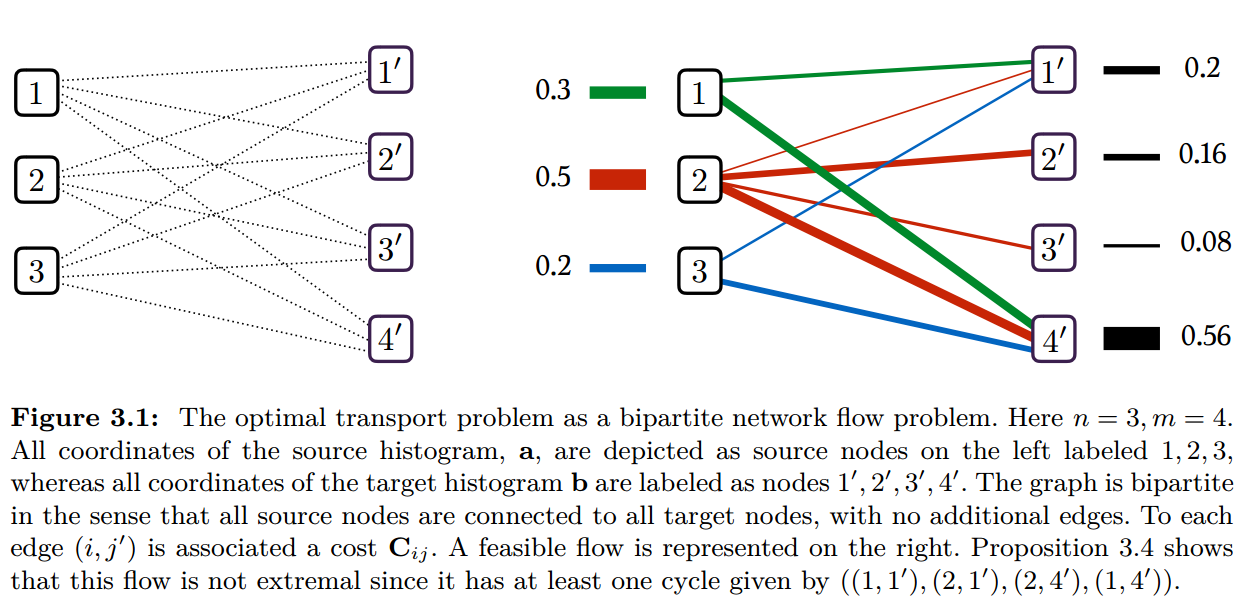
\includegraphics[scale = 0.3]{network_flow_problem.png}}
\end{minipage}
\caption{\footnotesize{\textbf{The optimal transport problem can be embedded to a graph to become the network flow problem}}}
\label{fig: network_flow_problem}
\end{figure}
\newpage
\section{$C$-transform}
Given the cost function $c$, we define the \textbf{c-transform (c-conjugate)} \citep{santambrogio2015optimal} as an extension to the concept of \emph{conjugate function} introduced in convex optimization \citep{rockafellar1970convex}. In fact, up to the change of sign, \underline{$c$-concavity} has exactly been defined as a generalization of convexity. 
\begin{definition}
Given a cost function $c: \cX \times \cY \rightarrow \bR_{+}$, $f: \cX \rightarrow \bR$, the \underline{\textbf{\emph{$c$-transform}}} of $f$ is defined as
\begin{align}
f^{c}(y) &:= \inf_{x\in \cX}c(x, y) - f(x)  \label{eqn: c_transform}
\end{align} The function $f^{c}: \cY \rightarrow \bR$ is also called the \underline{\textbf{\emph{$c$-conjugate function}}} of $f$. 

For discrete case, we have \textbf{\emph{$C$-transform vector}} for cost matrix $\mb{C} = [C_{i,j}]_{n \times m}$ and vector $\mb{f} = [f_1, \ldots, f_{n}] \in \bR^{n}$, 
\begin{align}
 \mb{f}_{j}^{\mb{C}} &:= \min_{i \in [1:n]}C_{i,j} - \mb{f}_{i} \label{eqn: c_transform_vector}
\end{align} The vector $\mb{f}^{\mb{C}} \in \bR^{m}$ is also called the \textbf{\emph{$C$-conjugate vector}} of $\mb{f}$.
\end{definition}

Similarly, since the cost function has two variables, we can define \textbf{$\bar{c}$-transform}
\begin{definition} 
Given a cost function $c: \cX \times \cY \rightarrow \bR_{+}$, $g: \cY \rightarrow \bR$, the \underline{\textbf{\emph{$\bar{c}$-transform}}} of $g$ is defined as
\begin{align}
g^{\bar{c}}(x) &:= \inf_{y\in \cY}c(x, y) - g(y)  \label{eqn: c_bar_transform}
\end{align} 

For discrete case, we have \textbf{\emph{$\bar{C}$-transform vector}} $\mb{g}^{\bar{\mb{C}}} \in \bR^{n}$ for cost matrix $\mb{C} = [C_{i,j}]_{n \times m}$ and vector $\mb{g} = [g_1, \ldots, g_{m}] \in \bR^{m}$, 
\begin{align}
 \mb{g}_{i}^{\bar{\mb{C}}} &:= \min_{j \in [1:m]}C_{i,j} - \mb{g}_{j} \label{eqn: c_bar_transform_vector}
\end{align}
\end{definition}
Note that $c$-transform or $\bar{c}$-transform can be obtained by \underline{\textbf{minimizing the dual objective}} \eqref{eqn: optimal_transport_dual_uncontrained} with respect to $\lambda$ or $\mu$, respectively while keeping the other one fixed.

Moreover, we can define $c$-concave and $\bar{c}$-concave functions
\begin{definition}
A function $\psi: \cX \rightarrow \bR$ is \textbf{$c$-concave} if there exists some function $\phi: \cY \rightarrow \bR$ and cost function $c: \cX \times \cY \rightarrow \bR_{+}$ so that $\psi$ is the $\bar{c}$-transform of $\phi$, i.e. 
$\psi = \phi^{\bar{c}}$. Denote $\psi$ as $c$-concave($\cX$)
\end{definition}
\begin{definition}
A function $\phi: \cY \rightarrow \bR$ is \textbf{$\bar{c}$-concave} if there exists some function $\psi: \cX \rightarrow \bR$ and cost function $c: \cX \times \cY \rightarrow \bR_{+}$ so that $\phi$ is the $c$-transform of $\psi$, i.e. 
$\phi = \psi^{c}$. Denote $\phi$ as $\bar{c}$-concave($\cY$)
\end{definition}
Note that a function is \underline{$c$-concave} means that it is the \underline{$\bar{c}$-transform} of some unknown function, and a function is \underline{$\bar{c}$-concave} means that is is the \underline{$c$-transform} of some unknown function. 

If $c=d$ is a distance function and $\cX = \cY$, due to symmetry, there is \textbf{no need to distinguish} $c$-transform vs. $\bar{c}$-transform (or $\bar{c}$-concave vs. $c$-concave). 


\subsection{Properties of c-transform}
c-transform plays an important role in dual representations. There are several properties:
\begin{itemize}
\item (for \textbf{distance metric} $c$, \textbf{no distinction} between $c$ and $\bar{c}$)\\
 If $c$ is defined as a distance, $\cX = \cY$, due to symmetry $\inf_{y\in \cY}c(x, y) - f(x) = \inf_{y\in \cY}c(x, y) - f(y)$ , thus $f^{c} = f^{\bar{c}}$.

\item The following inequality is for piecewise
 \begin{align*}
 \begin{array}{cc}
 i) \quad \mb{\lambda}_{1} \le \mb{\lambda}_{2} &\Leftrightarrow  \mb{\lambda}_{1}^{\mb{C}} \ge \mb{\lambda}_{2}^{\mb{C}} \\
ii) \quad \mb{\lambda}^{\mb{C}\bar{\mb{C}}} \ge \mb{\lambda}, &\quad  \mb{\mu}^{\bar{\mb{C}}\mb{C}} \ge \mb{\mu} \\
iii) \quad  \mb{\lambda}^{\mb{C}\bar{\mb{C}}\mb{C}} =  \mb{\lambda}^{\mb{C}} &
 \end{array}
\end{align*}
\begin{proof}
i) is from the definition of $C$-transform. Note that $\lambda_{1,j}^{\mb{C}} = \min_{i}C_{i,j} - \lambda_{1,i} \ge  \min_{i}C_{i,j} - \lambda_{2,i} = \lambda_{2,j}^{\mb{C}}$
ii) can be found by applying the definitoin twice:
\begin{align*}
\lambda_{i}^{\mb{C}\bar{\mb{C}}} &=\min_{j}C_{i,j} - \paren{ [\min_{i'}C_{i',j} - \lambda_{i'}]_{i'}}_{j} \\
&=\min_{j}\paren{C_{i,j} - \min_{i'}\paren{C_{i',j} - \lambda_{i'}}} \\
&\text{ since }\min_{i'}\paren{C_{i',j} - \lambda_{i'}} \le C_{i,j} - \lambda_{i}\\
&\ge \min_{j}\paren{C_{i,j} - \paren{C_{i,j} - \lambda_{i}}} \\
&= \min_{j}\paren{C_{i,j} - C_{i,j}} +  \lambda_{i} =  \lambda_{i}
\end{align*}
Similarly we can proof $\mb{\mu}^{\bar{\mb{C}\mb{C}}} \ge \mb{\mu}$

To proof iii), note that by ii) $ (\mb{\lambda}^{\mb{C}})^{\bar{\mb{C}}\mb{C}} \ge  \mb{\lambda}^{\mb{C}}$; Also by i) and ii) since $\mb{\lambda}^{\mb{C}\bar{\mb{C}}} \ge \mb{\lambda}$, then $(\mb{\lambda}^{\mb{C}\bar{\mb{C}}})^{\mb{C}}  \le \mb{\lambda}^{\mb{C}}$. Therefore $ \mb{\lambda}^{\mb{C}\bar{\mb{C}}\mb{C}} =  \mb{\lambda}^{\mb{C}}$.\qed
\end{proof}

This proof generalize to aribitrary function $f$ and its c-transform $f^{c}$ for all $x$ and $y$
\begin{proposition} 
Suppose that $c: \cX \times \cY \rightarrow \bR_{+}$ is real valued. 
\begin{enumerate}
\item For any $f_1: \cX \rightarrow \bR$ and $f_2: \cX \rightarrow \bR$, $f_{1} \le f_{2},\Leftrightarrow\;    f_{1}^{c} \ge f_{2}^{c}$
\item For any $f: \cX \rightarrow \bR$ and $g: \cY \rightarrow \bR$, $f^{c\bar{c}} \ge f, \;  g^{\bar{c}c} \ge g$ In general, $f^{c\bar{c}}$ is the \textbf{smallest $c$-concave function} larger than $f$
\item $f^{c\bar{c}c} =  f^{c}$ and $g^{\bar{c}c\bar{c}} =  g^{\bar{c}}$; in other words, $f^{c\bar{c}} = f$ if and only if $f$ is a $c$-concave function
\end{enumerate}
\end{proposition}



\item (\textbf{$c$-concavity} implies  a bound on the modulus of \textbf{continuity})
 \begin{proposition}\label{prop: c_concavity_lipschitz}
If $c: \cX \times \cX\rightarrow \bR$ is a distance, then the function $f: \cX \rightarrow \bR$ is \textbf{$c$-concave} if and only if $f$ is \textbf{Lipschitz continuous} with Lipschitz constant less than $1$ w.r.t. the distance $c$.  We will denote by $\text{Lip}_1$ the set of these functions. Moreover, for every $f \in \text{Lip}_1$, i.e. $\norm{f}{L} \le 1$, we have the $c$-transform of $f$, $f^{c} = -f$. \citep{santambrogio2015optimal}
\end{proposition}
\begin{proof}
$\Rightarrow$: since $f$ is $c$-concave, there exists some $g$ so that $f = g^{\bar{c}} = \inf_{y}c(x,y) - g(y)$. Note that the map $c_{y}: x\rightarrow c(x,y) \in \text{Lip}_1$  due to triangular inequality, and $c$ itself is the distance. Therefore $f \in \text{Lip}_1$ since the infimum of a family of Lipschitz continuous functions with the same
constant shares the same modulus of continuity. 

$\Leftarrow$: for $f \in  \text{Lip}_1$, we claim that $f(x) = \inf_{y}c(x,y) + f(y)$. To prove the claim, we see that $ \inf_{y}c(x,y) + f(y) \le  c(x,x) + f(x) = f(x)$ since $c(x,x) = 0$ for definiteness of distance $c$.

On the other hand, since  $f \in \text{Lip}_1$, therefore $f(x) -  f(y) \le \abs{f(x) -  f(y) } \le c(x, y)$. We have $f(x) \le c(x, y) + f(y)$ for all $y$. Taking infimum over $y$ at both sides, $f(x) \le \inf_{y}c(x, y) + f(y)$. Thus we prove that $f(x) = \inf_{y}c(x,y) + f(y)$. By definition of $c$-transform and $c$-concave, we have that $f = (-f)^{\bar{c}}$ so $f$ is  $c$-concave; Moreover, applying $-f \rightarrow f$ in the last formula, $f^{\bar{c}}=-f$, due to symmetry of $c$, $f^{c}=-f.$ \qed
\end{proof}
\end{itemize}

\subsection{Dual formulation with c-transform}
We present in this section an important property of the dual optimal transport problem \eqref{eqn: optimal_transport_dual_mat}. Note that by strong duality
\begin{align*}
L_{\mb{C}}(\mb{a}, \mb{b}) &= \max_{R(\mb{C})} \inn{\mb{\lambda}}{\mb{a}} + \inn{\mb{\mu}}{\mb{b}}
\end{align*} If we “freeze” the value of $\mb{\lambda}$, we can notice that there is no better vector solution for $\mb{\mu}$ than the \emph{\textbf{C-transform vector}} of $\mb{\lambda}$, denoted $\mb{\lambda}^{\mb{C}} \in \bR^m$.

Follwing the definition of C-transform vector \eqref{eqn: c_transform_vector}, we see that $\lambda_{i} + \lambda_{j}^{\mb{C}} \le C_{i,j}$ for all $i,j$. Therefore $(\mb{\lambda}, \mb{\lambda}^{\mb{C}}) \in R(\mb{C})$ is a feasible solution of dual problem. Moreover, $\mb{\lambda}^{\mb{C}}$ is the largest possible $\mu$ to satisfies the constraint. (since $\mb{\lambda} \oplus \mb{\lambda}^{\mb{C}} = \min_{i}\mb{C} \le \mb{C}$). Therefore 
\begin{align*}
 \inn{\mb{\lambda}}{\mb{a}} + \inn{\mb{\mu}}{\mb{b}} &\le  \inn{\mb{\lambda}}{\mb{a}} + \inn{ \mb{\lambda}^{\mb{C}}}{\mb{b}}
\end{align*} Thus the dual problem \eqref{eqn: optimal_transport_dual} is equivalent to an \textbf{unconstrained optimization problem}
\begin{align}
\max_{\mb{\lambda} \in \bR^{n}} & \inn{\mb{\lambda}}{\mb{a}} + \inn{\mb{\lambda}^{\mb{C}}}{\mb{b}} \label{eqn: optimal_transport_dual_c_transform}\end{align}
or using $\bar{C}$-transform vector
\begin{align}
\max_{\mb{\mu} \in \bR^{m}} & \inn{\mb{\mu}^{\bar{\mb{C}}}}{\mb{a}} + \inn{\mb{\mu}}{\mb{b}} \label{eqn: optimal_transport_dual_c_bar_transform}\end{align}

For probability measure we can write the dual formulation as
\begin{align}
\cL_{c}(\alpha, \beta)&:= \max_{\lambda \in \cC(\cX)} \E{X \sim \alpha}{\lambda(X)} + \E{Y \sim \beta}{\lambda^{c}(Y)}   \label{eqn: optimal_transport_dual_c_transform_prob} \\
&= \max_{\lambda \in c\text{-concave}(\cX)} \E{X \sim \alpha}{\lambda(X)} + \E{Y \sim \beta}{\lambda^{c}(Y)}   \label{eqn: optimal_transport_dual_c_concave_prob}
\end{align}



\newpage
\section{Wasserstein distance}
\subsection{Definition}
We can show that if $c(x,y)$ is a proper distance measure, then the optimal transport $\cL_{c}(\alpha, \beta)$ defines a divergence measure between the probability distribution $\alpha$ and $\beta$.

Here we can define the distance between between histograms supported on these bins
\begin{proposition}
We suppose $n = m$ and that for some $p \ge 1$, $\mb{C} = \mb{D}^p = [D_{i,j}^p]_{n\times n} \in \bR^{n \times n}$, where $
\mb{D} \in \bR_{+}^{n\times n}$ is a distance on $[1:n]$, i.e. 
\begin{enumerate}
\item $\mb{D} \in \bR_{+}^{n\times n}$ is symmetric; 
\item $D_{i,j} = 0$ iff  $i=j$;
\item (Triangular inequality): \; $D_{i,j} \le D_{i,k} + D_{k,j}$, for all $i,j,k \in [1:n]$
\end{enumerate}
Then the \underline{\textbf{$p$-Wasserstein distance}} $W_{p}(\mb{a}, \mb{b}) := L_{\mb{D}^{p}}(\mb{a}, \mb{b})^{\frac{1}{p}}$ is a distance between $\mb{a}, \mb{b} \in \Delta_{n}$, i.e. 
\begin{enumerate}
\item (Symmetric):\; $W_{p}(\mb{a}, \mb{b}) = W_{p}(\mb{b}, \mb{a})$
\item (Definiteness):\; $W_{p}(\mb{a}, \mb{b}) = 0 $ iff $\mb{a} = \mb{b}$
\item (Triangular inequality): \; $W_{p}(\mb{a}, \mb{b})  \le W_{p}(\mb{a}, \mb{c})  + W_{p}(\mb{c}, \mb{b}) $, for all $\mb{a}, \mb{b}, \mb{c} \in \Delta_{n}$.
\end{enumerate}
\end{proposition}
\begin{proof}
It is easy to show the symmetricity since the distance is symmetric thus the objective function is symmetric. The definiteness is shown by observing that $C_{i,i} = 0$, so the objective function $\sum_{i,j}C_{i,j}P_{i,j} = \sum_{i > j}C_{i,j}(P_{i,j} + P_{j,i}) > 0$, since $\sum_{j}P_{i,j} = a_{i} > 0$. If $\mb{a} = \mb{b}$, we choose $\mb{P} = \diag{\mb{a}} \in U(\mb{a}, \mb{a})$. We can show that $\diag{\mb{a}}  = \mb{P}^{*}$ since $\inn{\diag{\mb{a}}}{\mb{C}}  = \sum_{i > j}C_{i,j}(P_{i,j} + P_{j,i})  = 0$, when $P_{i,j} = P_{j,i} = 0$. Also $\inn{\mb{P}}{\mb{C}} \ge 0$ for all $\mb{a}$ $\mb{b}$ due to non-negativity of both $\mb{C}$ and $\mb{P}$. Therefore, $\inn{\diag{\mb{a}}}{\mb{C}} = W_{p}(\mb{a}, \mb{a}) = 0$.

To proof the triangular inequality, let $\mb{P} \in U(\mb{a}, \mb{c})$ and $\mb{Q} \in U(\mb{c}, \mb{b})$ be the optimal solution for $W_{p}(\mb{a}, \mb{c})$ and $W_{p}(\mb{c}, \mb{b})$. To avoid issues
that may arise from null coordinates in $\mb{c}$, we define a vector $\tilde{\mb{c}}$ such that $\tilde{c}_j := c_j$ if $c_j > 0$, and $\tilde{c}_j := 1$ otherwise, to write
\begin{align*}
\mb{S} &:= \mb{P}\diag{1/\tilde{\mb{c}}}\mb{Q} \in \bR_{+}^{n\times n},
\end{align*} We can show that $\mb{S} \in U(\mb{a}, \mb{b}).$
\begin{align*}
\mb{S}\mb{1}_{n} &=  \mb{P}\diag{1/\tilde{\mb{c}}}\mb{Q}\mb{1}_{n} \\
&=  \mb{P}\diag{1/\tilde{\mb{c}}}\mb{c} \qquad\qquad \text{ since } \mb{Q} \in U(\mb{c}, \mb{b})\\
&=  \mb{P}\mb{1}_{n}\qquad\qquad\text{ since each element is } c_{i}/c_{i} = 1\\ 
&= \mb{a}\qquad\qquad\text{ since } \mb{P} \in U(\mb{a}, \mb{c})
\end{align*} Similarly, $\mb{S}^{T}\mb{1}_{n} =\mb{b}$. 

Therefore, 
\begin{align*}
W_{p}(\mb{a}, \mb{b}) &= L_{\mb{D}^{p}}(\mb{a}, \mb{b})^{\frac{1}{p}} \\
& \le \inn{\mb{S}}{\mb{D}^{p}}^{\frac{1}{p}} \quad (\text{ optimality of LP}) \\
& =  \paren{\sum_{i,j}D^{p}_{i,j} \sum_{k} \frac{P_{i,k}Q_{k,j}}{c_{k}} }^{\frac{1}{p}}  =  \paren{\sum_{i,j,k}D^{p}_{i,j}\frac{P_{i,k}Q_{k,j}}{c_{k}} }^{\frac{1}{p}}\\
&\le  \paren{\sum_{i,j,k}\paren{D_{i,k} + D_{k,j}}^{p}\frac{P_{i,k}Q_{k,j}}{c_{k}} }^{\frac{1}{p}} \quad (\text{by triangular inequality of }D)\\
&\le  \paren{\sum_{i,j,k}D_{i,k}^{p}\frac{P_{i,k}Q_{k,j}}{c_{k}} }^{\frac{1}{p}} + \paren{\sum_{i,j,k}D_{k,j}^{p}\frac{P_{i,k}Q_{k,j}}{c_{k}} }^{\frac{1}{p}}  \quad (\text{by  Minkowski's inequality)} \\
&=  \paren{\sum_{i,k}D_{i,k}^{p}P_{i,k}\sum_{j}\frac{Q_{k,j}}{c_{k}} }^{\frac{1}{p}} + \paren{\sum_{j,k}D_{k,j}^{p}Q_{k,j}\sum_{i}\frac{P_{i,k}}{c_{k}} }^{\frac{1}{p}} \\
&\le  \paren{\sum_{i,k}D_{i,k}^{p}P_{i,k}\frac{c_{k}}{c_{k}} }^{\frac{1}{p}} + \paren{\sum_{j,k}D_{k,j}^{p}Q_{k,j}\frac{c_{k}}{c_{k}} }^{\frac{1}{p}}   \quad \text{since }\mb{Q} \in U(\mb{c}, \mb{b})\text{ and }\mb{P} \in U(\mb{a}, \mb{c}) \\
&= \paren{\sum_{i,k}D_{i,k}^{p}P_{i,k}}^{\frac{1}{p}} + \paren{\sum_{j,k}D_{k,j}^{p}Q_{k,j}}^{\frac{1}{p}} \\
& = W_{p}(\mb{a}, \mb{c}) + W_{p}(\mb{c}, \mb{b}). \quad \text{since }\mb{Q},\mb{P}\text{ are optimal solutions.}
\end{align*} which concludes the proof. \qed
\end{proof}
Note  that for $1> p\ge 0$, $\mb{D}^{p}$ is a distance. It implies that while for $p \ge 1$, $\cW_p(\alpha, \beta)$ is a distance, in the case $0 < p \le 1$, it is actually
$\cW_p(\alpha, \beta)^p$ which defines a distance on the simplex.



We can generalize the definition of \textbf{Wasserstein distance to aribitrary measure} $\cX = \cY$ that defines a distance $d$. 
\begin{proposition}
We suppose $\cX = \cY$ and that for some $p \ge 1$, $c(x,y)= d(x,y)^p$, where $d$ is a distance on $\cX$, i.e. 
\begin{enumerate}
\item $d(x, y) = d(y, x)$ for all $x, y\in \cX$; 
\item $d(x, y)  = 0$ iff  $x=y$;
\item (Triangular inequality): \; $d(x, y) \le d(x, z) + d(z, y)$, for all $x, y, z \in \cX$
\end{enumerate}
Then the \underline{\textbf{$p$-Wasserstein distance}} on $\cX$, $\cW_{p}(\alpha, \beta) := \cL_{d^{p}}(\alpha, \beta)^{\frac{1}{p}}$ is a valid distance between $\alpha, \beta \in \cM_{+}^{1}(\cX)$, i.e. 
\begin{enumerate}
\item (Symmetric):\; $\cW_{p}(\alpha, \beta) = \cW_{p}( \beta, \alpha)$ for all $\alpha, \beta \in  \cM(\cX)$
\item (Definiteness):\; $\cW_{p}(\alpha, \beta) = 0 $ iff $\alpha = \beta$
\item (Triangular inequality): \; $\cW_{p}(\alpha, \beta)  \le \cW_{p}(\alpha, \gamma)  + \cW_{p}(\gamma, \beta) $, for all $\alpha, \beta, \gamma \in \cM_{+}^{1}(\cX)$.
\end{enumerate}
\end{proposition}


\subsection{Basic properties of Wasserstein distance}
Note that 
\begin{itemize}
\item Wasserstein distance $\cW_{p}(\alpha, \beta)$ is a distance between two Radon measures $\alpha$, $\beta$ on $\cX$. 
\item The general optimal transport problem in \eqref{eqn: optimal_transport_continuous} and \eqref{eqn: optimal_transport_linear_prog} does not require that $c=d$ is distance matrix. That is the \textbf{Wasserstein distance} is the optimal value of a \underline{\textbf{special case}} in \textbf{optimal transport problem}. 
\item Wasserstein distance, or Optimal Transport (OT), $\cW_{p}(\alpha, \beta)$ depends on the \emph{distance definition} $d$ on the \textbf{\emph{base} measure} $\cX$. In other word, OT can be seen as automatically "\underline{\textbf{lifting}}" a \underline{\emph{ground metric}} in $\cX$ to a \emph{metric} between \textbf{\emph{measures}} on $\cX$

\item One of most \textbf{important} propery of Wasserstein distance is that  it is a \emph{\textbf{weak distance}}, i.e. it allows one to compare singular distributions (for instance, discrete ones) whose \textbf{supports \emph{do not overlap}} and to quantify the spatial shift between the supports of two distributions. 

In fact, $\cW_{p}$ is a way to quantify the \underline{\emph{\textbf{weak convergence}}} or \emph{convergence in distribution (in law)} \citep{villani2009optimal}: 
\begin{definition} (\textbf{Weak Convergence or Convergence in distribution})
On a compact domain $\cX$ , $(\alpha_k)_k$ converges \textbf{weakly} to $\alpha$ in $\cM_{+}^{1}(\cX)$ (denoted $\alpha_{n}\stackrel{d}{\rightarrow} \alpha$) if and only if \emph{for any \textbf{continuous} function} $g \in \cC(\cX)$, $\int_{\cX} g d\alpha_k \rightarrow \int_{\cX} g d\alpha$. One needs to add additional decay conditions on $g$ on noncompact domains. 

This notion of weak convergence corresponds to the \textbf{convergence in the distribution} of random vectors. Note the any random variable $X_{n}$ is a continous function on $\Omega$, and its distribution is the push-forward measure $\alpha_{n} = X_{n\#}\bP$. Therefore, $\alpha_{n}\stackrel{d}{\rightarrow} \alpha$  is equivalent to $X_{n}\stackrel{d}{\rightarrow} X$.

This convergence can be shown to be equivalent to $\cW_{p}(\alpha_{n}, \alpha) \rightarrow 0$ [Villani, 2009, Theorem 6.8]. Thus we can also write the weak convergance as $\alpha_{n}\stackrel{\cW_{p}}{\rightarrow} \alpha$.
\end{definition}


\item (\textbf{Translation}): A nice feature of the Wasserstein distance over a Euclidean space $\cX = \bR^d$ for the $\ell^2$-distance ground cost $c(x, y) = \norm{x - y}{2}^2$ is that one can \emph{\textbf{factor out} translations}. Define the translation operator $T_{\tau}: x \rightarrow x-\tau$. Then 
\begin{align}
\cW_{p}(T_{\tau_1 \#}\alpha, \,T_{\tau_{2} \#} \beta)^2 &= \cW_{p}(\alpha, \beta)^2 -2 \inn{\tau_1 - \tau_{2}}{\mb{m}_{\alpha} - \mb{m}_{\beta}} + \norm{\tau_1 - \tau_{2}}{2}^2 \label{eqn: translation_wasserstein_dis}
\end{align} where $\mb{m}_{\alpha} := \int_{\cX} x d\alpha(x) \in \bR^{d}$ is the barycenter of  the measure $\alpha$ (in prob. the mean of random variable $X$). This interpretation is intuitive, since the translation operator moves the barycenter of the mass, thus the distance need to take into account of the difference between two barycenters. 

In particular, this implies the nice \textbf{decomposition} of the distance as
\begin{align}
\cW_{p}(\alpha, \beta)^2 &= \cW_{p}(\tilde{\alpha}, \,\tilde{\beta})^2  + \norm{\mb{m}_{\alpha} - \mb{m}_{\beta}}{2}^2 \label{eqn: translation_wasserstein_dis2}
\end{align} where $\tilde{\alpha} = T_{\mb{m}_{\alpha} \#}\alpha$ and $\tilde{\beta} = T_{\mb{m}_{\beta} \#}\beta$ are the centered measures with zero mean.
\end{itemize}


\subsection{Brenier theorem: Monge-Kantorovich equivalence}
\begin{itemize}
\item  \begin{remark}
\emph{\textbf{Brenier theorem}} shows that in $\bR^d$ for $p = 2$, (i.e. $\cW_{2}$) if at least one of the two input measures has a \emph{density}, and for measures with \emph{second order moments}, then the \emph{\textbf{Kantorovich and Monge problems are equivalent}}.  That is the non-convex optimal assignment problem in \eqref{eqn: optimal_assignment_cont} and the convex optimal transport problem in \eqref{eqn: optimal_transport_continuous} have the same optimal solution and the Kantorovich relaxation is \textbf{tight}. Note that we have already shown in section \ref{sec: discrete_tight} that in discrete case, these two problems are equivalent when the permutation matrix is the optimal coupling matrix. Brenier's theorem is for arbitrary measures.
\end{remark}

\item \begin{theorem} (\textbf{Brenier})\\ 
In the case $\cX = \cY = \bR^d$ and $c(x, y) = \norm{x -y}{2}^2$, if at least one of the two input measures (denoted $\alpha$) has a density $\rho_{\alpha}$ with respect to
the Lebesgue measure, then the optimal $\pi$ in the Kantorovich formulation \eqref{eqn: optimal_transport_continuous} is \textbf{unique} and is \textbf{supported} on the graph $(\mb{x}, T(\mb{x}))$ of a "\textbf{Monge map}" $T : \bR^d \rightarrow \bR^d$. This means that $\pi = (\text{Id}, T)_{\#}\alpha$, i.e. 
\begin{align}
\forall\, h\in \cC(\cX \times \cY), \quad \int_{\cX \times \cY} h (x, y) d\pi(x, y) &= \int_{\cX} h(x, T(x)) d\alpha(x).  \label{eqn: Brenier_theorem}
\end{align} Furthermore, this map $T$ is uniquely defined as the \textbf{gradient} of a \textbf{convex function} $\phi$, $T(x) = \grad{}{\phi(x)}$, where $\phi$ is the \textbf{unique} (up to an additive constant) \textbf{convex} function such that $(\grad{}{\phi})_{\#}\alpha = \beta$. This convex function is related to the \textbf{dual potential} $\lambda(\cdot)$ solving \eqref{eqn: optimal_transport_dual_cont} as $\phi(x) = \frac{1}{2}\norm{x}{2}^2 - \lambda(x)$, $\text{Id}(\cdot)$ is an identity mapping.
\end{theorem}
\begin{proof}
We sketch the main ingredients of the proof; more proof can be found in \citep{santambrogio2015optimal, figalli2021invitation}.

We mark that the $c(x, y) = \norm{x -y}{2}^2$ has decomposition $c(x, y) = \norm{x}{2}^2 + \norm{y}{2}^2 - 2 \inn{x}{y}$. Therefore,  $\int c(x,y) d\pi(x, y) = C_{\alpha, \beta} - 2 \int  \inn{x}{y}d\pi(x, y)$ where the constant is $C_{\alpha, \beta} = \int \norm{x}{2}^2 d\alpha(x) + \int \norm{y}{2}^2 d\beta(y)$. Instead of solving the primal problem \eqref{eqn: optimal_transport_continuous}, one solves 
\begin{align*}
\max_{\pi \in \cM_{+}^{1}(\cX \times \cY)}& \int_{\cX \times \cY} \inn{x}{y} d \pi(x, y)   \\
\text{s.t. }& P_{\cX \#}\pi = \alpha,  \nonumber \\
& P_{\cY \#}\pi = \beta  \nonumber
\end{align*} This problem has a dual problem 
\begin{align*}
 \min_{(\phi,  \psi) \in \in \cC(\cX)\times \cC(\cY)} & \int_{\cX}\phi(x) d\alpha(x) + \int_{\cY}\psi(y) d\beta(y) \\
\text{s.t. }&  \phi(x) + \psi(y) \ge \inn{x}{y},\quad \forall x\in \cX, y \in \cY,
\end{align*} The relation between $(\phi,  \psi)$ and $(\lambda, \mu)$ is that $\phi(\cdot) = \frac{1}{2}\norm{\cdot}{2}^2 - \lambda(\cdot)$ and $\psi(\cdot) = \frac{1}{2}\norm{\cdot}{2}^2 - \mu(\cdot)$, respectively. One can replace the constraint above by
\begin{align}
\psi(y) \ge \phi^{*}(y) := \sup_{x}\inn{x}{y} - \phi(x) \label{eqn: Brenier_conjugate}
\end{align} $\phi^{*}$ is the \textbf{Legendre transform} (or, Fenchel's \underline{\emph{\textbf{conjugate function}}}) of $\phi$ and is a \textbf{convex function} as a supremum of linear forms \citep{rockafellar1970convex}. Since the objective appearing in dual form above is linear and the integrating measures positive, one can \emph{\textbf{minimize}} explicitly with respect to $\psi$ and set $\psi = \phi^{*}$ in order to consider the unconstrained problem 
\begin{align}
\min_{\phi\in \cC(\cX)} & \int_{\cX}\phi(x) d\alpha(x) + \int_{\cY}\phi^{*}(y) d\beta(y) \label{eqn: Brenier_dual}
\end{align} since the objective function in \eqref{eqn: Brenier_dual} is the lower bound of the original dual objective above with $\psi = \phi^{*}$ as a feasible solution, maximizing this problem will be equivalent to maximizing the original dual objective.  By iterating this argument twice, one can replace $\phi$ by $\phi^{**}$, which is a \textbf{convex function}, and thus impose in \eqref{eqn: Brenier_dual} that \underline{$\phi$ is convex}. Therefore
\begin{align*}
\inf_{\pi \in \cM_{+}^{1}(\cX \times \cY)} \int_{\cX \times \cY} -\inn{x}{y} d \pi(x, y) &\ge \sup_{\phi(x) + \psi(y) \ge \inn{x}{y}}\int_{\cX}-\phi(x) d\alpha(x) + \int_{\cY}-\psi(y) d\beta(y) \\
&\ge \sup_{\phi \text{ convex}}\int_{\cX}-\phi(x) d\alpha(x) + \int_{\cY}-\phi^{*}(y) d\beta(y)
\end{align*}

Note that the support of $\pi$ is bounded by the equality condition
\begin{align}
\text{Supp}(\pi)  \subset \set{(x, y) \in \cX \times \cY:  \lambda(x) + \phi^{*}(y) = \inn{x}{y}},
\end{align} which shows that such a $y$ is optimal for the minimization \eqref{eqn: Brenier_conjugate} of the Legendre transform, whose optimality condition reads
$y \in \partial \phi(x)$, the \emph{\textbf{sub-differential}} of $\phi$ \citep{rockafellar1970convex}. 

Since $\phi$ is convex, it is \emph{differentiable} everywhere,  and since $\alpha$ has a density, it is also differentiable \emph{$\alpha$-almost everywhere}.  This shows that for each $x$, the associated $y$ is \textbf{uniquely} defined \emph{$\alpha$-almost everywhere} as $y = \grad{}{\phi}(x)$, and it shows that necessarily $\pi = (\text{Id}, \grad{}{\phi})_{\#}\alpha$.
\qed
\end{proof}

\item  \begin{remark}
Brenier's theorem, stating that an optimal transport map must be the \textbf{gradient of a convex function}, provides a useful generalization of the notion of increasing functions in dimension more than one. This is the main reason why optimal transport can be used to define \textbf{quantile functions} in \emph{arbitrary dimensions}, which is in turn useful for applications to \emph{\textbf{quantile regression} problems}.
\end{remark}

\item 
From the proof, we see that when $\cX = \cY = \bR^d$ and $c(x, y) = \norm{x -y}{2}^2$ there exists an alternative dual problem \eqref{eqn: Brenier_dual}. The probabilistic interpretation for \eqref{eqn: Brenier_dual} is
\begin{align}
\min_{\phi\in \cC(\cX)} & \E{X \sim \alpha}{\phi(X)} +  \E{Y \sim \beta}{\phi^{*}(Y)} \label{eqn: Brenier_dual_prob}
\end{align}
\end{itemize}

\subsection{Dual Formulation of Wasserstein Distance}
\begin{itemize}
\item \begin{theorem} (\textbf{Kantorovich-Rubenstein duality}) \citep{villani2009optimal}\\
Let $\cX$ be a \textbf{Polish space}, i.e. $\cX$ a complete separable metric space equipped with a Borel $\sigma$-algebra induced by metric $d$, and $\alpha$ and $\beta$ be Borel measures on $\cX$. Let $Lip_1$ be the space of all 
$1$-\textbf{Lipschitz} functions $f: \cX \to \bR$ with respect to metric $d$  such that
\begin{align*}
\norm{f}{L}  := \sup_{x, y \in \cX}\set{\frac{\abs{f(x) - f(y)}}{d(x, y)}} \le 1.
\end{align*}
Then the Wasserstein distance between $\alpha$ and $\beta$ induced by $d$ can be obtained by the following optimization problem
\begin{align}
\cW_{d}(\alpha, \beta) &= \sup_{f \in Lip_1}\set{\int_{\cX} f d\alpha  - \int_{\cX} f d\beta}. \label{eqn: wass_dist_dual}
\end{align} 
\end{theorem}

\item \begin{remark}
Note here the we use $\mu(y)=\inf_{x}d(x,y) - \lambda(x)$ and since $\norm{\lambda}{L} \le 1$, this implies $g(y)= - f(y)$. This theorem in the basis for Wasserstein GAN algorithm using 1-Wasserstein distance $\cW_1$ \citep{arjovsky2017wasserstein}.
\end{remark}
\end{itemize}

\section{Examples of Wasserstein distance}
\subsection{Wasserstein distance between discrete measures}
\begin{itemize}
\item (\textbf{discrete measures with $\ell_1$} as ground metric)\\
For two discrete measures $\alpha = \sum_{i=1}^{n}a_i \delta_{\mb{x}_{i}}$ and $\beta := \sum_{i=1}^{n}b_i \delta_{\mb{y}_{i}}$,  
\begin{align}
\cW_{1}(\alpha, \beta) = \norm{\mb{a} - \mb{b}}{1},  \label{eqn: wass_dist_l1_discrete}
\end{align} i.e. $L_{\mb{C}}(\mb{a}, \mb{b})= \norm{\mb{a} - \mb{b}}{1}$ where $\mb{C} = \mb{1}\mb{1}^{T} - \mb{I}.$

\item (\textbf{discrete measures with binary cost} as ground metric)\\
For two discrete measures $\alpha \in \cM_{+}(\cX)$ and $\beta \in \cM_{+}(\cX)$, and $c(x, y)$ is $0$ if $x = y$ and $1$ when $x \neq y$, 
\begin{align*}
\cW_{1}(\alpha, \beta) = \text{TV}(\alpha, \beta)
\end{align*} where $\text{TV}(\alpha, \beta)$ is the total variation distance between two measures.

\item (\textbf{discrete empirical measures with }$\ell_p$ as ground metric)\\
Consider two empirical measures on $\cX = \bR$, $\alpha_{n} = \frac{1}{n}\sum_{i=1}^{n}\delta_{x_{i}}$ and $\beta_{n} := \frac{1}{n}\sum_{i=1}^{n}\delta_{y_{i}}$. Assuming (without loss of generality) that the points are \emph{\textbf{ordered}}, i.e. $x_1 \le x_2 \le \ldots \le x_n$ and $y_1 \le y_2 \le  \ldots  \le y_n$, then one has the simple formula
\begin{align}
\cW_{p}(\alpha_{n}, \beta_{n})^{p} =\frac{1}{n} \sum_{i}^{n}\abs{x_i - y_i}^{p} = \norm{\mb{x}- \mb{y}}{p}^{p} := (d_{p}(\mb{x}, \mb{y}))^{p} \label{eqn: wass_dist_lp_discrete}
\end{align} which is the $\ell^{p}$ norm between two vectors of ordered values of $\alpha_n$ and $\beta_n$. That statement is valid only \emph{\textbf{locally}}, in the
sense that the \emph{order} (and those vector representations) \emph{might change} whenever some of the values change. 
\end{itemize}

\subsection{$p$-Wasserstein distance on 1-dimensional real line $\bR$}
\begin{itemize}
\item (\textbf{Wasserstein distance on real line} $\bR$)\\
Define the \emph{\textbf{cumulative distribution function}} $F_{\alpha}(t):= \int_{-\infty}^{t}d\alpha := \bP(X \in (-\infty, t])$ for measure $\alpha \in \cM(\bR)$ and corresponding random variable $X$. Then the pseudoinverse $F_{\alpha}^{-1}: [0,1] \rightarrow \bR\cup\set{-\infty}$
\begin{align}
F_{\alpha}^{-1}(r) &:= \min_{x}\set{x \in \bR\cup\set{-\infty}: \; F_{\alpha}(x) \ge r}\quad \label{eqn: quantile}
\end{align} That function is also called the \underline{\textbf{generalized quantile function}} of $\alpha$. 

Then
\begin{align}
\cW_{p}(\alpha, \beta)^{p} = \norm{F_{\alpha}^{-1} - F_{\beta}^{-1}}{p}^{p} := \int_{0}^{1}\norm{F_{\alpha}^{-1}(r) - F_{\beta}^{-1}(r)}{p}^{p} dr \label{eqn: wass_dist_lp_general}
\end{align} where the norm $\norm{F_{\alpha}^{-1} - F_{\beta}^{-1}}{p}$ is $L^{p}$-norm on functionals. 

This means that through map $\alpha \rightarrow F_{\alpha}^{-1}$, the Wasserstein distance is isometric to a \emph{linear space equipped with the $L^p$ norm} or, equivalently, that the \textbf{Wasserstein distance for measures on the \underline{1-dimensional} real line $\bR$ is a \underline{\emph{Hilbertian metric}}}.

\begin{figure}
\begin{minipage}[t]{1\linewidth}
  \centering
  \centerline{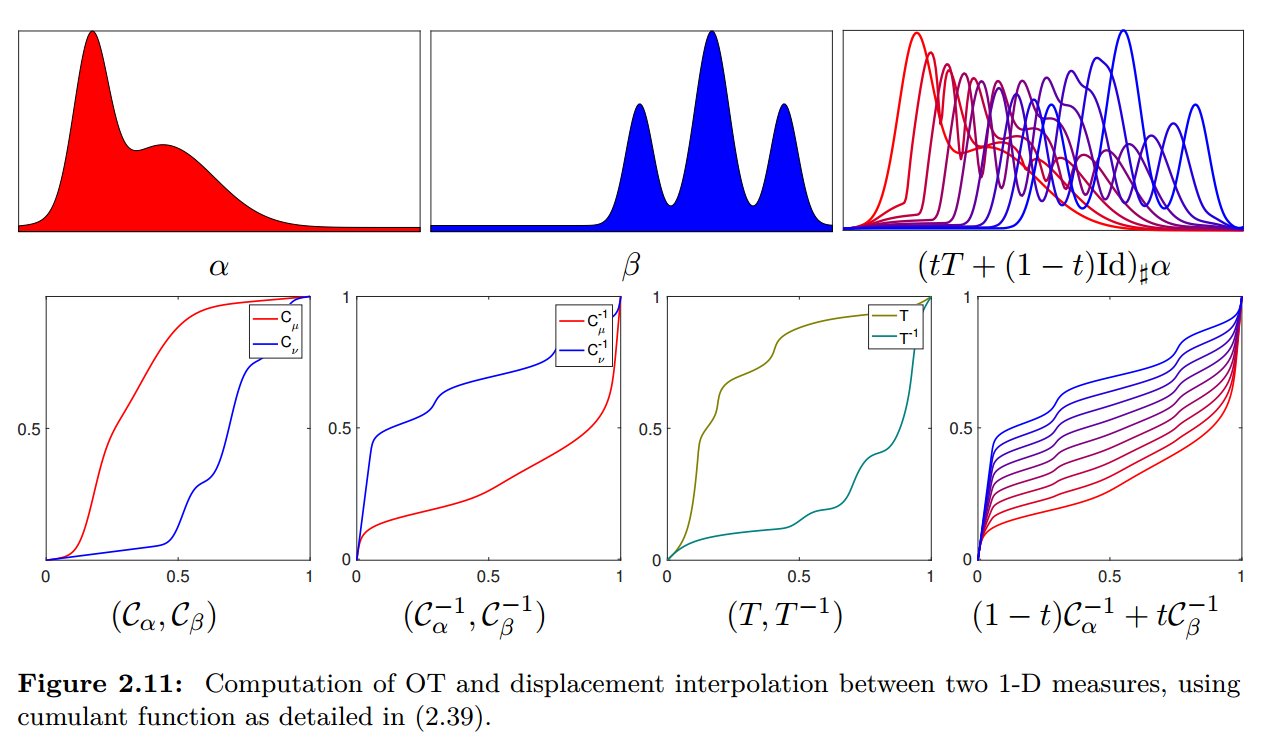
\includegraphics[scale = 0.3]{1d_wass_dist_opt_map.png}}
\end{minipage}
\caption{\footnotesize{\textbf{The interpolation between two 1-D measures, using cumulant function and quantile functions}}}
\label{fig: 1d_wass_dist_opt_map}
\end{figure}
\end{itemize}

\subsection{1-Wasserstein distance $\cW_1$}
\begin{itemize}
\item $\cW_1$ is also called the \textbf{earth mover’s distances (EMD)}.

\item ($\cW_1$ on $\bR$ is a \textbf{norm} and is equal to \textbf{Total Variation distance})\\

Following \eqref{eqn: wass_dist_lp_general}, when $p=1$, it further simplifies as 
\begin{align}
\cW_{1}(\alpha, \beta) &=  \norm{F_{\alpha} - F_{\beta}}{1} := \int_{-\infty}^{\infty}\norm{F_{\alpha}(x) - F_{\beta}(x)}{1} dx  \label{eqn: wass_dist_l1_general}\\
&=  \int_{-\infty}^{\infty}\abs{\int_{-\infty}^{x}d(\alpha - \beta) } \label{eqn: wass_dist_l1_general_tv0}
\end{align} which shows that $\cW_1$ on $\bR$ is a \textbf{norm}. An optimal Monge map $T$ such that $T_{\#}\alpha = \beta$ is then defined by
\begin{align}
T = F_{\beta}^{-1} \circ  F_{\alpha}    \label{eqn: wass_dist_l1_general_optimal_map}
\end{align}

\item (\textbf{$p$-Wasserstein distance is related to Lipschitz continous function f})\\
As a result of \textbf{Proposition} \ref{prop: c_concavity_lipschitz}, The $p$-Wasserstein distance can also be written as 
\begin{align}
\cW_{p}(\alpha, \beta) &:= \inf_{\pi \in U(\alpha, \beta)}\set{\int_{\cX \times \cX}d_{p}(x,y) d\pi(x, y)} \nonumber\\
&= \sup_{f \in \text{Lip}_1}\set{\int_{M} f(x) d(\alpha - \beta)(x) }  \label{eqn: wass_dist_c_transform_lip1}
\end{align} This results can be extended to $\cW_{p}$
\begin{align}
\cW_{p}(\alpha, \beta) &= \sup_{f \in \text{Lip}_p}\set{\int_{M} f(x) d(\alpha - \beta)(x) }  \label{eqn: wass_dist_p_lip}
\end{align} where 
\begin{align*}
 \text{Lip}_p &= \set{f: \sup_{x\neq y} \frac{\abs{f(x) - f(y)}}{d(x, y)^{p}} \le 1}
\end{align*} This is equivalent to stating that $\cW_{p}$ is the dual of $p$-H\"older functions. 

If $\cX = \cY = \bR^{d}$,  the global Lipschitz constraint appearing in \eqref{eqn: wass_dist_c_transform_lip1} can be made local as a uniform bound on the \emph{\textbf{gradient} of} $f$,
\begin{align}
\cW_{1}(\alpha, \beta) &= \sup_{\norm{\grad{}{f}}{\infty} \le 1}\set{\int_{M} f(x) d(\alpha - \beta)(x) }  \label{eqn: wass_dist_norm_f} \\
&= \inf_{s}\set{\int_{\bR^{d}} \norm{s(x)}{2}dx:  \text{div}(s) = \alpha - \beta }  \label{eqn: wass_dist_beckmann}
\end{align} The latter is  an optimization problem under fixed \emph{\textbf{divergence}} constraint, which is often called the \textbf{\emph{Beckmann formulation}}. Here the vectorial function $s(\mb{x}) \in \bR^2$ can be interpreted as a flow field, describing locally the movement of mass. Outside the support of the two input measures,  $\text{div}(s) = 0$, which is the conservation of mass constraint. Once properly discretized using finite elements, Problems \eqref{eqn: wass_dist_norm_f} and \eqref{eqn: wass_dist_beckmann} become nonsmooth convex optimization problems. 

\item (\textbf{Concentration inequality of $p$-Wasserstein distance}) 
\begin{definition}\citep{wainwright2019high} For a given metric $d$, the \emph{probability measure} $\bP$ is said to satisfy a \textbf{$d$-transportation cost inequality} with parameter $\gamma > 0$ if
\begin{align}
\cW_{p}(\bQ, \bP) &\le \sqrt{2 \gamma \kl{\bQ}{\bP}},  \label{eqn: wasserstein_inequality}
\end{align}  for all \emph{probability measures} $\bQ$.
\end{definition}

\begin{definition}\citep{wainwright2019high} The concentration function $\alpha: [0, \infty) \rightarrow  \bR_{+}$ associated with metric
measure space $(\bP, \cX, d)$ is given by
\begin{align}
\alpha_{\bP,(\cX,d)}(\epsilon) &:= \sup_{A \subseteq \cX }\set{1- \bP\{x\in \cX: d(x, A) < \epsilon\} \Big| \bP\{A\} \ge \frac{1}{2}},  \label{eqn: concentration_function}
\end{align} where the supremum is taken over all measurable subsets $A \subseteq \cX$.
\end{definition}

\begin{theorem}(From transportation cost to concentration \citep{wainwright2019high}) Consider a metric measure space $(\bP, \cX, d)$, and suppose that $\bP$ satisfies the $d$-transportation cost inequality \eqref{eqn: wasserstein_inequality}. Then its concentration function satisfies the bound
\begin{align}
\alpha_{\bP,(\cX,d)}(t) &\le 2\exp\paren{-\frac{t^2}{2 \gamma}}.  \label{eqn: wasserstein_concentration_1}
\end{align}
Moreover, for any $X \sim \bP$ and any $L$-Lipschitz function $f : \cX \rightarrow \bR$, we have the concentration inequality
\begin{align}
\bP\set{\abs{f(X)  - \E{}{f(X)} } \ge t} &\le 2\exp\paren{-\frac{t^2}{2 \gamma L^2}} \label{eqn: wasserstein_concentration_2}
\end{align}
\end{theorem}

\end{itemize}

\subsection{Wasserstein distance between Gaussian measures}
\begin{itemize}
\item Given $\alpha = \cN(\mb{m}_{\alpha}, \mb{\Sigma}_{\alpha})$ and $\beta = \cN(\mb{m}_{\beta}, \mb{\Sigma}_{\beta})$ are two Guassian measures on $\bR^{d}$, the push-forward operator $T$ can be defined as a linear map
\begin{align}
T(\mb{x}) &= \mb{m}_{\beta} + \mb{A}\paren{\mb{x} - \mb{m}_{\alpha}} \label{eqn: gaussian_push_forward}\\
\text{where }&\mb{A} := \mb{\Sigma}_{\alpha}^{-\frac{1}{2}}\paren{ \mb{\Sigma}_{\alpha}^{\frac{1}{2}}\mb{\Sigma}_{\beta}\mb{\Sigma}_{\alpha}^{\frac{1}{2}}}^{\frac{1}{2}}\mb{\Sigma}_{\alpha}^{-\frac{1}{2}} \nonumber
\end{align} where $\mb{A}$ is symmetric and positive definite. We can show that $T_{\#}\alpha = \beta$ and $T$ is the optimal transport map.
\begin{proof}
Note that the density after push-forward
\begin{align*}
\rho_{\beta}(T(\mb{x})) &= \det\paren{2\pi\abs{\mb{\Sigma}_{\beta}}}^{-\frac{1}{2}}\exp\set{-\frac{1}{2}\paren{T(\mb{x}) - \mb{m}_{\beta}}^{T}\mb{\Sigma}_{\beta}^{-1}\paren{T(\mb{x}) - \mb{m}_{\beta}} } \\
&= \det\paren{2\pi\abs{\mb{\Sigma}_{\beta}}}^{-\frac{1}{2}}\exp\set{-\frac{1}{2}\paren{\mb{A}\paren{\mb{x} - \mb{m}_{\alpha}}}^{T}\mb{\Sigma}_{\beta}^{-1}\paren{\mb{A}\paren{\mb{x} - \mb{m}_{\alpha}}} } \\
&=  \det\paren{2\pi\abs{\mb{\Sigma}_{\beta}}}^{-\frac{1}{2}}\exp\set{-\frac{1}{2}\paren{\mb{x} - \mb{m}_{\alpha}}^{T}\paren{\mb{A}^{T}\mb{\Sigma}_{\beta}^{-1}\mb{A}}\paren{\mb{x} - \mb{m}_{\alpha}} } \\
&= \det\paren{2\pi\abs{\mb{\Sigma}_{\beta}}}^{-\frac{1}{2}}\exp\set{-\frac{1}{2}\paren{\mb{x} - \mb{m}_{\alpha}}^{T}\tilde{\mb{\Sigma}}^{-1}\paren{\mb{x} - \mb{m}_{\alpha}} }\\
\text{where }\tilde{\mb{\Sigma}}^{-1}&=\paren{ \mb{\Sigma}_{\alpha}^{-\frac{1}{2}}\paren{ \mb{\Sigma}_{\alpha}^{\frac{1}{2}}\mb{\Sigma}_{\beta}\mb{\Sigma}_{\alpha}^{\frac{1}{2}}}^{\frac{1}{2}}\paren{\mb{\Sigma}_{\alpha}^{\frac{1}{2}} \mb{\Sigma}_{\beta} \mb{\Sigma}_{\alpha}^{\frac{1}{2}}}^{-1}\paren{ \mb{\Sigma}_{\alpha}^{\frac{1}{2}}\mb{\Sigma}_{\beta}\mb{\Sigma}_{\alpha}^{\frac{1}{2}}}^{\frac{1}{2}}\mb{\Sigma}_{\alpha}^{-\frac{1}{2}} } \\
&=\mb{\Sigma}_{\alpha}^{-1}\\
\rho_{\beta}(T(\mb{x})) &= \det\paren{2\pi\abs{\mb{\Sigma}_{\beta}}}^{-\frac{1}{2}}\exp\set{-\frac{1}{2}\paren{\mb{x} - \mb{m}_{\alpha}}^{T}\mb{\Sigma}_{\alpha}^{-1}\paren{\mb{x} - \mb{m}_{\alpha}} }
\end{align*} and since $T$ is a linear map, the Jacobian
\begin{align*}
\abs{\det{T'(x)}} &= \abs{\det{A}} = \abs{\frac{\det{\mb{\Sigma}_{\beta}}}{\det{\mb{\Sigma}_{\alpha}}}}^{\frac{1}{2}}
\end{align*} which means $\rho_{\alpha} = \abs{\det{T'(x)}}\rho_{\beta}(T(\mb{x}))$, therefore $T_{\#}\alpha = \beta$.

Also note that $T$ is the \emph{gradient} of the \emph{convex} (quadratic) function $\phi(\mb{x}) = \frac{1}{2}\paren{\mb{x} - \mb{m}_{\alpha}}^{T}\mb{A}\paren{\mb{x} - \mb{m}_{\alpha}} + \inn{\mb{m}_{\beta}}{\mb{x}}$, which is the potential function of the dual. By Brenier's theorem, that $T$ is optimal. \qed
\end{proof}

Therefore, we can find the \textbf{2-Wasserstein distance between two Gaussian measures} as 
\begin{align}
\cW_{2}(\alpha, \beta)^2 &=  \cW_{2}( \cN(\mb{m}_{\alpha}, \mb{\Sigma}_{\alpha}), \cN(\mb{m}_{\beta}, \mb{\Sigma}_{\beta}))^2 \nonumber\\
&= \norm{\mb{m}_{\alpha} - \mb{m}_{\beta}}{2}^{2} + \cB\paren{\mb{\Sigma}_{\alpha}, \mb{\Sigma}_{\beta}}^2 \label{eqn: 2_wasserstein_gaussian}
\end{align} Note that this uses the \emph{translation interpolation} formula in \eqref{eqn: translation_wasserstein_dis2}. The second term is called \underline{\emph{\textbf{Bures metric}}}. It is defined as 
\begin{align}
\cB\paren{\mb{\Sigma}_{\alpha}, \mb{\Sigma}_{\beta}}^2 &= \tr{\mb{\Sigma}_{\alpha} + \mb{\Sigma}_{\beta} - 2\paren{ \mb{\Sigma}_{\alpha}^{\frac{1}{2}}\mb{\Sigma}_{\beta}\mb{\Sigma}_{\alpha}^{\frac{1}{2}}}^{\frac{1}{2}}}.  \label{eqn: bures_metric}
\end{align} Bures metric is the distance between two positive definite matrices. $\cB\paren{\mb{\Sigma}_{\alpha}, \mb{\Sigma}_{\beta}}^2$ is also \textbf{convex} with respect to both its arguments.

If both Gaussian measuers have independent coordinates $\mb{\Sigma}_{\alpha} = \diag{\lambda_{\alpha,1}, \ldots, \lambda_{\alpha,n}}$ and $\mb{\Sigma}_{\beta} = \diag{\lambda_{\beta,1}, \ldots, \lambda_{\beta,n}}$, then the Bures metric is the \textbf{Hellinger distance}
\begin{align}
\cB\paren{\mb{\Sigma}_{\alpha}, \mb{\Sigma}_{\beta}} &= \norm{\sqrt{\mb{\lambda}_{\alpha}} - \sqrt{\mb{\lambda}_{\beta}}}{2}. \label{eqn: bures_metric_independent}
\end{align}

For a detailed treatment of the Wasserstein geometry of Gaussian distributions, we refer to \citep{takatsu2011wasserstein}, and for additional considerations
on the Bures metric the reader can consult the very recent references \citep{malago2018wasserstein, bhatia2019bures}.

\begin{figure}
\begin{minipage}[t]{1\linewidth}
  \centering
  \centerline{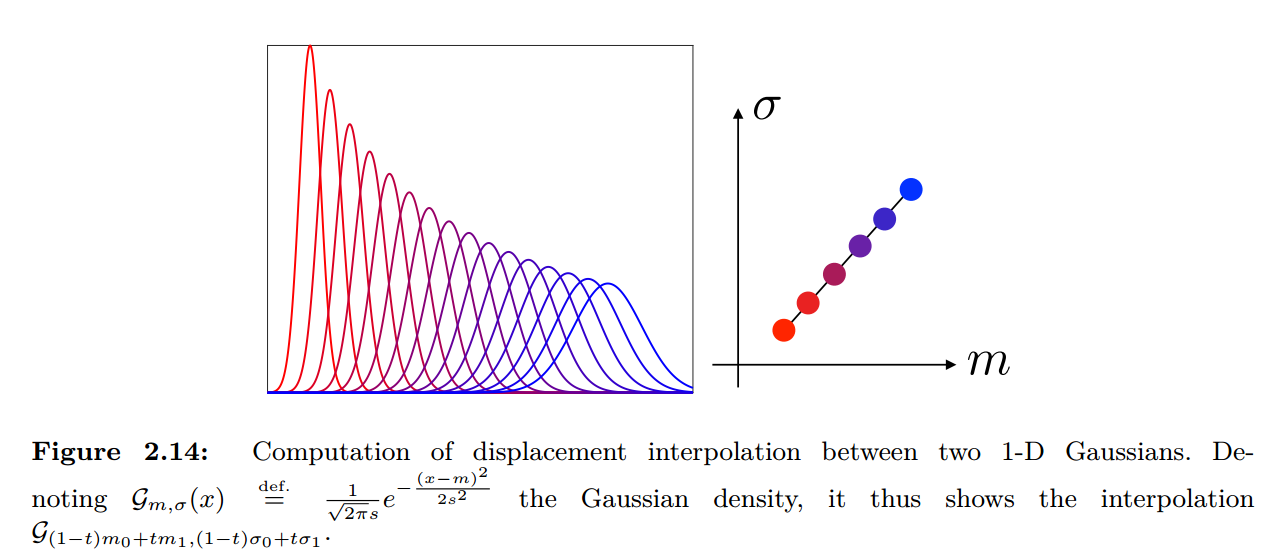
\includegraphics[scale = 0.35]{gaussian_displacement.png}}
\end{minipage}
\caption{\footnotesize{\textbf{Computation of displacement interpolation between two 1-D Gaussians.}}}
\label{fig: gaussian_displacement}
\end{figure}

\end{itemize}

\newpage
\bibliographystyle{plainnat}
\bibliography{book_reference.bib}
\end{document}